\documentclass[10pt]{article}\usepackage[]{graphicx}\usepackage[]{color}
%% maxwidth is the original width if it is less than linewidth
%% otherwise use linewidth (to make sure the graphics do not exceed the margin)
\makeatletter
\def\maxwidth{ %
  \ifdim\Gin@nat@width>\linewidth
    \linewidth
  \else
    \Gin@nat@width
  \fi
}
\makeatother

\definecolor{fgcolor}{rgb}{0.345, 0.345, 0.345}
\newcommand{\hlnum}[1]{\textcolor[rgb]{0.686,0.059,0.569}{#1}}%
\newcommand{\hlstr}[1]{\textcolor[rgb]{0.192,0.494,0.8}{#1}}%
\newcommand{\hlcom}[1]{\textcolor[rgb]{0.678,0.584,0.686}{\textit{#1}}}%
\newcommand{\hlopt}[1]{\textcolor[rgb]{0,0,0}{#1}}%
\newcommand{\hlstd}[1]{\textcolor[rgb]{0.345,0.345,0.345}{#1}}%
\newcommand{\hlkwa}[1]{\textcolor[rgb]{0.161,0.373,0.58}{\textbf{#1}}}%
\newcommand{\hlkwb}[1]{\textcolor[rgb]{0.69,0.353,0.396}{#1}}%
\newcommand{\hlkwc}[1]{\textcolor[rgb]{0.333,0.667,0.333}{#1}}%
\newcommand{\hlkwd}[1]{\textcolor[rgb]{0.737,0.353,0.396}{\textbf{#1}}}%
\let\hlipl\hlkwb

\usepackage{framed}
\makeatletter
\newenvironment{kframe}{%
 \def\at@end@of@kframe{}%
 \ifinner\ifhmode%
  \def\at@end@of@kframe{\end{minipage}}%
  \begin{minipage}{\columnwidth}%
 \fi\fi%
 \def\FrameCommand##1{\hskip\@totalleftmargin \hskip-\fboxsep
 \colorbox{shadecolor}{##1}\hskip-\fboxsep
     % There is no \\@totalrightmargin, so:
     \hskip-\linewidth \hskip-\@totalleftmargin \hskip\columnwidth}%
 \MakeFramed {\advance\hsize-\width
   \@totalleftmargin\z@ \linewidth\hsize
   \@setminipage}}%
 {\par\unskip\endMakeFramed%
 \at@end@of@kframe}
\makeatother

\definecolor{shadecolor}{rgb}{.97, .97, .97}
\definecolor{messagecolor}{rgb}{0, 0, 0}
\definecolor{warningcolor}{rgb}{1, 0, 1}
\definecolor{errorcolor}{rgb}{1, 0, 0}
\newenvironment{knitrout}{}{} % an empty environment to be redefined in TeX

\usepackage{alltt}

\usepackage{amsmath,amssymb,amsthm}
\usepackage{fancyhdr,url,hyperref}
\usepackage{graphicx,xspace}
\usepackage{subfigure}
\usepackage{tikz}
\usetikzlibrary{arrows,decorations.pathmorphing,backgrounds,positioning,fit,through}

\oddsidemargin 0in  %0.5in
\topmargin     0in
\leftmargin    0in
\rightmargin   0in
\textheight    9in
\textwidth     6in %6in
%\headheight    0in
%\headsep       0in
%\footskip      0.5in

\newtheorem{thm}{Theorem}
\newtheorem{cor}[thm]{Corollary}
\newtheorem{obs}{Observation}
\newtheorem{lemma}{Lemma}
\newtheorem{claim}{Claim}
\newtheorem{definition}{Definition}
\newtheorem{question}{Question}
\newtheorem{answer}{Answer}
\newtheorem{problem}{Problem}
\newtheorem{solution}{Solution}
\newtheorem{conjecture}{Conjecture}

\pagestyle{fancy}

\lhead{\textsc{Prof. McNamara}}
\chead{\textsc{SDS/MTH 220: Lecture notes}}
\lfoot{}
\cfoot{}
%\cfoot{\thepage}
\rfoot{}
\renewcommand{\headrulewidth}{0.2pt}
\renewcommand{\footrulewidth}{0.0pt}

\newcommand{\ans}{\vspace{0.25in}}
\newcommand{\R}{{\sf R}\xspace}
\newcommand{\cmd}[1]{\texttt{#1}}
\newcommand{\Ex}{\mathbb{E}}

\rhead{\textsc{November 20, 2017}}
\IfFileExists{upquote.sty}{\usepackage{upquote}}{}
\begin{document}

\paragraph{Agenda}
\begin{enumerate}
  \itemsep0em
  \item The Bootstrap
\end{enumerate}


\paragraph{Warumup: 4.39 -- Coffee, depression, and physical activity} Caffeine is the world's most widely used stimulant, with approximately 80\% consumed in the form of coffee. However, studies that analyze the relationship between coffee / caffeine consumption and depression risk are scarce. Since depression is also known to have an association with physical activity, participants in a study investigating the relationship between coffee consumption and depression were asked to report the number of hours they spent per week on moderate (e.g., brisk walking) and vigorous (e.g., strenuous sports and jogging) exercise. Based on these data the researchers estimated the total hours of metabolic equivalent tasks (MET) per week, a value always greater than 0. The table below gives summary statistics of MET for women in this study based on the amount of coffee consumed. 
 
\begin{center}
\begin{tabular}{l  r  r  r  r  r  r}
\multicolumn{1}{c}{}  & \multicolumn{5}{c}{\textit{Caffeinated coffee consumption}} \\
\cline{2-6}
				& $\le$ 1 cup/week	& 2-6 cups/week	& 1 cup/day	& 2-3 cups/day & $\ge$ 4 cups/day & Total	\\
\hline
Mean			& 18.7	& 19.6	& 19.3	& 18.9	& 17.5 			  \\
SD				& 21.1	& 25.5	& 22.5	& 22.0	& 22.0 \\
$n$				& 12,215	& 6,617 		& 17,234	& 12,290	& 2,383 	& 50,739 \\
\hline
\end{tabular}
\end{center}

\begin{enumerate}
  \itemsep0.4in
\item Write the hypotheses for evaluating if the average physical activity level varies among the different levels of coffee consumption.

\item Check conditions and describe any assumptions you must make to proceed with the test.

\item Below is part of the output associated with this test. Fill in the empty cells.

\begin{center}
\begin{tabular}{lrrrrr}
  \hline
 			& Df 	& Sum Sq		& Mean Sq	& F value	& Pr($>$F) \\ 
  \hline
coffee	 	& \fbox{\textcolor{white}{{\footnotesize XXXXX}}}	 & \fbox{\textcolor{white}{{\footnotesize XXXXX}}} 		& \fbox{\textcolor{white}{{\footnotesize XXXXX}}} 			& \fbox{\textcolor{white}{{\footnotesize XXXXX}}} 	& 0.0003 \\ 
Residuals		& \fbox{\textcolor{white}{{\footnotesize XXXXX}}} & 25,564,819 	& \fbox{\textcolor{white}{{\footnotesize  XXXXX}}} 			&  		&  \\ 
   \hline
Total			& \fbox{\textcolor{white}{{\footnotesize XXXXX}}} &25,575,327
\end{tabular}
\end{center}

\item What is the conclusion of the test?

\item Given that the overall mean is 19, write out the three different forms of the model
\vspace{1.5in}

\end{enumerate}







  
\paragraph{The Bootstrap}

The bootstrap is a powerful computational technique for estimating all kinds of things. [Do not believe the hyperbolic warnings in Section 4.5.3 of the book!] It is particularly useful when our actual data sample is non-normal. 

  \begin{itemize}
  \item The bootstrap works in three steps:
  \begin{enumerate}
    \item Construct a sample of $n$ items from your original data set, sampling \emph{with replacement} ({\tt resample()})
    \item Compute the statistic of interest on this sample (in our case, the mean ({\tt mean()}))
    \item Repeat this process many, many times and collect the results ({\tt do()})
  \end{enumerate}
  \item This \emph{bootstrap distribution} is an approximation of the sampling distribution of your statistic
  \item Big Idea: The middle $P$\% of the bootstrap distribution makes a $P$\% confidence interval for the statistic in question, without making many assumptions about the distribution of $X$!
\end{itemize}

\paragraph{Wage example}

Consider the following sample of 534 hourly wages from the Current Population Survey (of 1985): 

\begin{knitrout}\footnotesize
\definecolor{shadecolor}{rgb}{0.969, 0.969, 0.969}\color{fgcolor}\begin{kframe}
\begin{alltt}
\hlkwd{favstats}\hlstd{(}\hlopt{~}\hlstd{wage,} \hlkwc{data} \hlstd{= CPS85)}
\end{alltt}
\begin{verbatim}
##  min   Q1 median    Q3  max     mean       sd   n missing
##    1 5.25   7.78 11.25 44.5 9.024064 5.139097 534       0
\end{verbatim}
\end{kframe}
\end{knitrout}


\paragraph{Distributional assumptions}
\begin{enumerate}
\item Construct a 95\% confidence interval for the mean wage in the 1985 CPS, based on this sample. Assume that $5.139$ is the true population standard deviation, and that wages are normally distributed.
\begin{knitrout}\footnotesize
\definecolor{shadecolor}{rgb}{0.969, 0.969, 0.969}\color{fgcolor}\begin{kframe}
\begin{alltt}
\hlstd{x.bar} \hlkwb{=} \hlkwd{mean}\hlstd{(}\hlopt{~}\hlstd{wage,} \hlkwc{data}\hlstd{=CPS85)}
\hlstd{sd} \hlkwb{=} \hlkwd{sd}\hlstd{(}\hlopt{~}\hlstd{wage,} \hlkwc{data}\hlstd{=CPS85)}
\hlstd{n} \hlkwb{=} \hlkwd{nrow}\hlstd{(CPS85)}
\hlstd{z.star} \hlkwb{=} \hlkwd{qnorm}\hlstd{(}\hlkwd{c}\hlstd{(}\hlnum{0.025}\hlstd{,} \hlnum{0.975}\hlstd{))}
\hlstd{se} \hlkwb{=} \hlstd{sd} \hlopt{/} \hlkwd{sqrt}\hlstd{(n)}
\hlstd{x.bar} \hlopt{+} \hlstd{z.star} \hlopt{*} \hlstd{se}
\end{alltt}
\begin{verbatim}
## [1] 8.588186 9.459941
\end{verbatim}
\end{kframe}
\end{knitrout}
  
  \item Using the $t$-statistic below, construct a 95\% confidence interval for the mean wage that makes no assumption about the population standard deviation, but assumes that wages are normally distributed.

\begin{knitrout}\footnotesize
\definecolor{shadecolor}{rgb}{0.969, 0.969, 0.969}\color{fgcolor}\begin{kframe}
\begin{alltt}
\hlkwd{qt}\hlstd{(}\hlnum{0.975}\hlstd{,} \hlkwc{df} \hlstd{= n}\hlopt{-}\hlnum{1}\hlstd{)}
\end{alltt}
\begin{verbatim}
## [1] 1.964425
\end{verbatim}
\begin{alltt}
\hlstd{t.star} \hlkwb{=} \hlkwd{qt}\hlstd{(}\hlkwd{c}\hlstd{(}\hlnum{0.025}\hlstd{,} \hlnum{0.975}\hlstd{),} \hlkwc{df}\hlstd{=n}\hlopt{-}\hlnum{1}\hlstd{)}
\hlstd{x.bar} \hlopt{+} \hlstd{t.star} \hlopt{*} \hlstd{se}
\end{alltt}
\begin{verbatim}
## [1] 8.587194 9.460933
\end{verbatim}
\end{kframe}
\end{knitrout}

  \item Examine the distribution of $wage$. Is it normally distributed? 
\begin{knitrout}\footnotesize
\definecolor{shadecolor}{rgb}{0.969, 0.969, 0.969}\color{fgcolor}\begin{kframe}
\begin{alltt}
\hlkwd{densityplot}\hlstd{(}\hlopt{~}\hlstd{wage,} \hlkwc{data}\hlstd{=CPS85)}
\end{alltt}
\end{kframe}
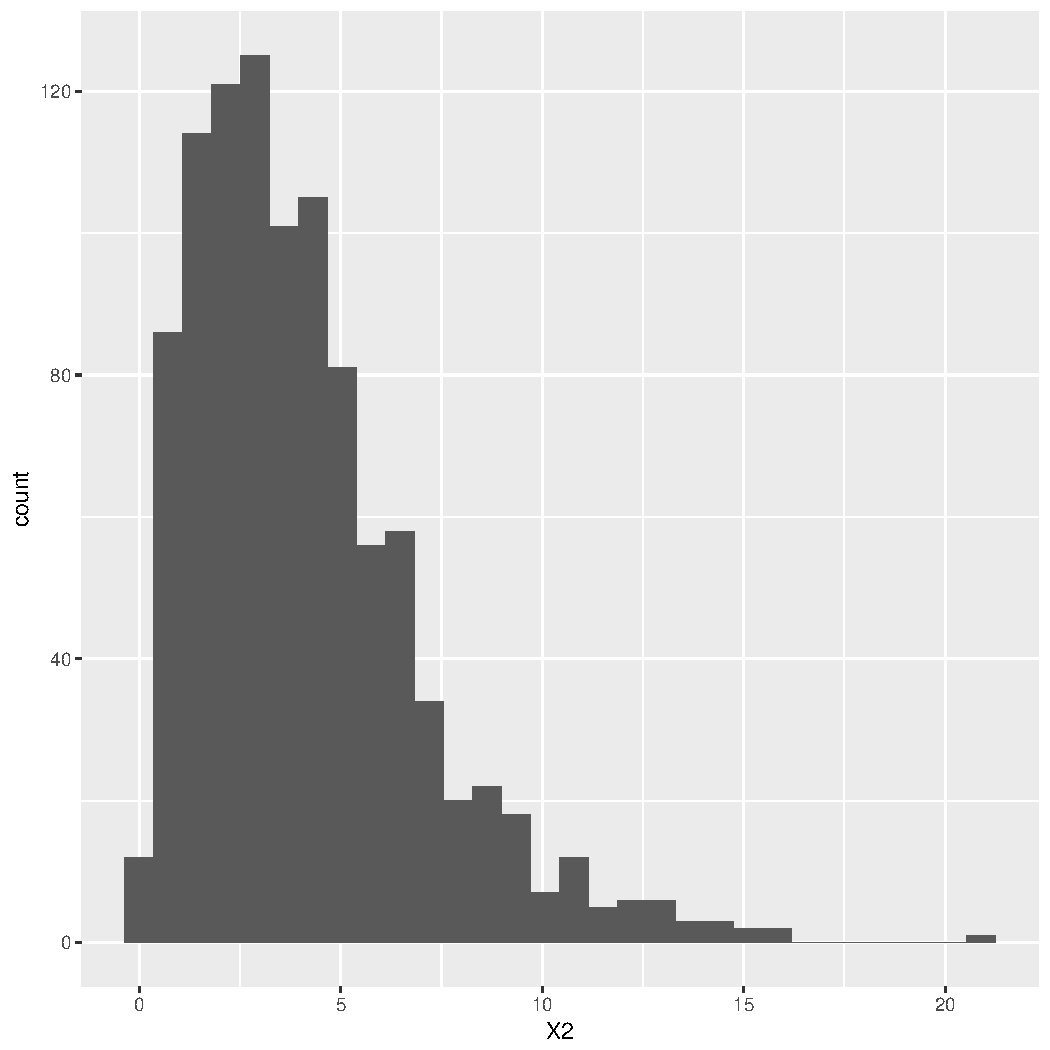
\includegraphics[width=\maxwidth]{figure/unnamed-chunk-5-1} 

\end{knitrout}
\end{enumerate}

\paragraph{The bootstrap} Using the bootstrap, construct a 95\% confidence interval for the mean wage that does not assume that wages are normally distributed.
\begin{knitrout}\footnotesize
\definecolor{shadecolor}{rgb}{0.969, 0.969, 0.969}\color{fgcolor}\begin{kframe}
\begin{alltt}
\hlstd{bstrap} \hlkwb{<-} \hlkwd{do}\hlstd{(}\hlnum{10000}\hlstd{)} \hlopt{*} \hlkwd{mean}\hlstd{(}\hlopt{~}\hlstd{wage,} \hlkwc{data} \hlstd{=} \hlkwd{resample}\hlstd{(CPS85))}
\hlkwd{qdata}\hlstd{(}\hlopt{~}\hlstd{mean,} \hlkwc{p} \hlstd{=} \hlkwd{c}\hlstd{(}\hlnum{0.025}\hlstd{,} \hlnum{0.975}\hlstd{),} \hlkwc{data} \hlstd{= bstrap)}
\end{alltt}
\begin{verbatim}
##       quantile     p
## 2.5%  8.596251 0.025
## 97.5% 9.462125 0.975
\end{verbatim}
\end{kframe}
\end{knitrout}
Compare the three confidence intervals you constructed. Do you see any important differences?
  

%' \newpage
%' 
%' \paragraph{Instructor's Notes}
%' 
%' \paragraph{Solution to 4.39}
%' 
%' 
%' \begin{enumerate}
%' 
%' \item $H_0$: The mean MET for each group is equal to each other.
%' \[ \mu_{\le \text{1 cup/week}} = \mu_{\text{2-6 cups/week}} = \mu_{\text{1 cup/day}} = \mu_{\text{2-3 cups/day}} = \mu_{\ge \text{4 cups/day}} \]
%' $H_A$: At least one pair of means is different.
%' 
%' \item The conditions that need to be satisfied for ANOVA are:
%' \begin{enumerate}
%' \item Independence: We don't have any information on how the data were collected, so we cannot assess independence. To proceed, we must assume the subjects in each group are independent.
%' \item Approximately normal: The data are bound below by zero and the standard deviations are larger than the means, indicating very strong strong skew. However, since the sample sizes are extremely large, even extreme skew is acceptable.
%' \item Constant variance: This condition appears to be met, standard deviations are pretty consistent across groups.
%' \end{enumerate}
%' In order to proceed with the test we will need to assume independence. 
%' 
%' \item $\:$ \\
%' 
%' {\scriptsize
%' \begin{center}
%' \renewcommand{\arraystretch}{1.25}
%' \begin{tabular}{lrrrrr}
%'   \hline
%'    		& Df 	& Sum Sq		& Mean Sq	& F value	& Pr($>$F) \\ 
%'   \hline
%' coffee	 	& \fbox{{{\footnotesize 5 - 1 = 4}}}	 & \fbox{{{\footnotesize 25575327 - 25564819 = 10508}}} 		& \fbox{{{\footnotesize 10508 / 4 = 2627}}} 			& \fbox{{{\footnotesize 2627 / 505 = 5.2}}} 	& 0.0003 \\ 
%' Residuals		& \fbox{{{\footnotesize 50739 - 5 = 50734}}} & 25564819 	& \fbox{{{\footnotesize  25564819 / 50624 =  505}}} 			&  		&  \\ 
%'    \hline
%' Total			& \fbox{{{\footnotesize 50739 - 1 = 50738}}} & 25575327
%' \end{tabular}
%' \end{center}
%' }
%' 
%' \item Since p-value is low, reject $H_0$. The data provide convincing evidence that the average MET differs between at least one pair of groups.
%' 
%' \end{enumerate}
%' 
%' 
%' \paragraph{Motivation for the Bootstrap}
%' 
%' \begin{itemize}
%'   \item Thus far, we've constructed confidence intervals for the population mean of the form
%'   $$
%'     \bar{x} \pm z^* \cdot \frac{\sigma_X}{\sqrt{n}} \, ,
%'   $$
%'   where $\sigma_X$ was known, and our sample size ($n$) was large enough that the CLT implied a reasonably normal sampling distribution of the mean. 
%'   \item In reality, we rarely know $\sigma_X$, so we approximate it with $s$, the standard deviation of the sample. This leads to confidence intervals of the form
%'   $$
%'     \bar{x} \pm t^* \cdot \frac{s}{\sqrt{n}} \, ,
%'   $$
%'   where $t^*$ is a value from the $t$-distribution (accessed in R by {\tt \{p, q, r, d\}t()}).
%'   \item The $t$-distribution is similar to the Normal distribution (unimodal, symmetric), but is indexed by an additional parameter (the degrees of freedom), and has fatter tails. In fact, the $t$-distribution converges to the Normal for an infinite sample size (i.e. $t(\mu, \sigma, \infty) = N(\mu, \sigma)$). [More on this in Chapter 7.]
%'   \item But this procedure still assumes that $X$ is normally distributed, and forces the confidence intervals to be symmetric. 
%'   \item Question: Is there a way to ditch all of the theory, make almost no assumptions about the data we've collected, and still find a reasonably accurate confidence interval? 
%'   \end{itemize}
%' 
%' \paragraph{Solution to Bootstrap Exercises}
%' 
%' \begin{enumerate}
%' 
%'   \item Normal based interval:
%'   
%'   <<fig.show='hide'>>=
%' x.bar = mean(~wage, data=CPS85)
%' sd = sd(~wage, data=CPS85)
%' n = nrow(CPS85)
%' z.star = qnorm(c(0.025, 0.975))
%' se = sd / sqrt(n)
%' x.bar + z.star * se
%' plotDist("norm", params = list(mean = x.bar, sd = se), lwd=5)
%' @
%' 
%'   \item $t$-based interval:
%'   
%'     <<fig.show='hide'>>=
%' t.star = qt(c(0.025, 0.975), df=n-1)
%' x.bar + t.star * se
%' densityplot(~wage, data=CPS85)
%' @
%' 
%' 
%'   \item Bootstrap interval:
%'   
%' <<fig.show='hide'>>=
%' bstrap = do(10000) * mean(~wage, data=resample(CPS85))
%' qdata(c(0.025, 0.975), vals=mean, data=bstrap)
%' densityplot(~mean, data=bstrap, lwd=5)
%' @
%'   
%'   \end{enumerate}

\end{document}
